\chapter{Realizacja}
W celu rozpoznania przechodnia został użyty połączony obraz termowizyjny (IR) i kolorowy (RGB) nazywany dalej RGBIR. Następnie ten obraz zostaje poddany analizie HOG oraz klasyfikacji za pomocą SVM. W celu ustalenia obszaru zainteresowania na obrazie termowizyjnym za pomocą wzorca probabilistycznego zostają wytypowani kandydaci.

\section{Akwizycja obrazu}
Obraz kolorowy służy jako obraz bazowy. Rozdzielczości 640 x 480 pikseli, prędkością 30 klatek na sekundę i głębi 8 bitów na kanał. Źródłem tego obrazu jest kamera podłączona do układu za pomocą interfejsu HDMI. Na obraz bazowy zostaje nałożony obraz termowizyjny z kamery Lepton, który różni się znacząco parametrami. Abu je zsynchronizować zastosowano bufor ramki, do którego jest zapisywany obraz z prędkością 9 klatek na sekundę a odczytywany z prędkością 30. Kolejnym przekształceniem jest transformacja projekcyjna. Ma na celu powiększenie i dopasowanie obrazu by poprawnie pokrywał się z obraz wizyjnym. W tym celu został zaimplementowany moduł który oblicza na podstawie parametrów macierzy transformaty i koordynatami piksela obrazu źródłowego odpowiadającą mu pozycję na obrazie termowizyjnym zapisanym w buforze ramki. Następny moduł dokonuje interpolacji dwuliniowej. Do poprawnej interpolacji wymagane są 4 piksele otaczające obliczony z projekcji punkt. W celu zredukowania liczby dostępów do pamięci i zwiększenie szybkość działania moduł zapamiętuje 4 ostatnio użyte wartości pikseli. Rozwiązanie to pozwala na pracę w czasie rzeczywistym małym kosztem zasobów układu.
Strumień wizyjny jak i termowizyjny działają w AXI-Stream. Umożliwia to łatwą synchronizację obu obrazów na podstawie sygnału SOF (ang. Start o frame). Moduł synchronizacji czeka na pojawienie się tego sygnału w strumieniu termowizyjnym. Do tego momentu wszystkie napływające piksele są odrzucane. Gdy pojawi się sygnał strumień IR zostaje zatrzymany i czeka na pojawienie się sygnału SOF w bazowym strumieniu wizyjnym. Po jego wykryciu strumień IR rusza. Oba strumienie zostają zsynchronizowane tworząc strumień wizyjna obrazu RGBIR. Następnie ten strumień zostaje przesłany do pamięci za pośrednictwem VDMA oraz (po koloryzacji i nałożeniu) wyświetlony na monitorze przez port VGA.

\section{Kalibracja}
Aby obraz termowizyjny poprawnie pokrywał się z obrazem RGB należy wykonać procedurę kalibracji. Kalibracja przeprowadzana jest ręcznie. Oprogramowanie kamery pozwala na zapisanie na karcie SD specjalnego obrazu kalibracyjnego w którym jest zawarty zrzut aktualnie wyświetlanego obrazu wraz z nieprzetworzonym projekcyjnie obrazem IR. Następnie w pakiecie Matlab zostaje obliczona macierz transformaty projekcyjnej za pomocą wbudowanej funkcji. Wymaga ona wskazania 4 par odpowiadających sobie punktów na obrazie RGB oraz IR. Nową macierz można wgrać podając jej parametry w konsoli. 


\section{Wyznaczanie ROI}
Strumień IR z kamery zostaje zbinearyzowany i zbadany w detektorze DPM kożystającym z wzorca probabilistycznego. Moduł DPM przesyła do pamięci listę koordynatów kandydatów wraz z mocą dopasowania. Moduł DPM został zaczerpnięty z pracy inżynierskiej. Moduł wykorzystuję strumień bezpośrednio z kamery. Wielkość okna detekcji wynosi 16 x 40 pikseli. Jeżeli badany obraz binarny wykazał odpowiedni poziom dopasowania do wzorca zostaje wysłana o tym informacja poprzez AXI-Stream do pamięci. Informacja zawiera koordynaty okna w układzie odniesienia kamery IR oraz wartość mocy dopasowania. Gdy zostanie zbadane ostatnie okno w obrazie zostaje wysłany sygnał TLAST co wygeneruje przerwanie dla systemu procesorowego.

\section{Klasyfikacja za pomcą SVM}
Z lisy kandydatów wygenerowanej przez moduł DPM wybierany jest wynik o najwyższej mocy dopasowania. Koordynaty z układu odniesienia kamery zostają poddane transformacie projekcyjnej do układu odniesienia kamery RGB. Z obszaru na obrazie RGBIR zawierającym potencjalnie człowieka zostają wyodrębnione cechy HOG które następnie służą jako wektor dla SVM.

Klasyfikator został opracowany i nauczony na podstawie 60 wyselekcjonowanych obrazów. 30 z nich stanowiło próbką pozytywną zawierającą osobę a 30 nie. Nauczanie zostało zrealizowane przy użyciu oprogramowania Matlab. Próbki pozytywne zostały wygenerowane poprzez zapis ROI wyznaczonych przez wzorzec probabilistyczny. 

\section{Prezentacja wyników}
Na wyjściu konsoli zostają podane współrzędne oraz moc dopasowania i klasyfikacja obiektu. Na obrazie wyjściowym VGA obszar ten zostaje zaznaczony zieloną ramką. Jeżeli potencjalny obszar nie został zakwalifikowany jako człowiek ale miał największą moc dopasowania DPM to obszar zostaję zaznaczony czerwoną ramką. Czarna ramka oznacza że nie został wykryty żaden obiekt. 

Mając do dyspozycji układ heterogeniczny rodziny Zynq-7000 od firmy Xilinx operacje zostały podzielone między programowalną logiką a systemem procesorowym. Ogólny zarys systemu został przedstawiony na rysunku \ref{fig:systemwizyjny}.

\begin{figure}[h]
    \centering
    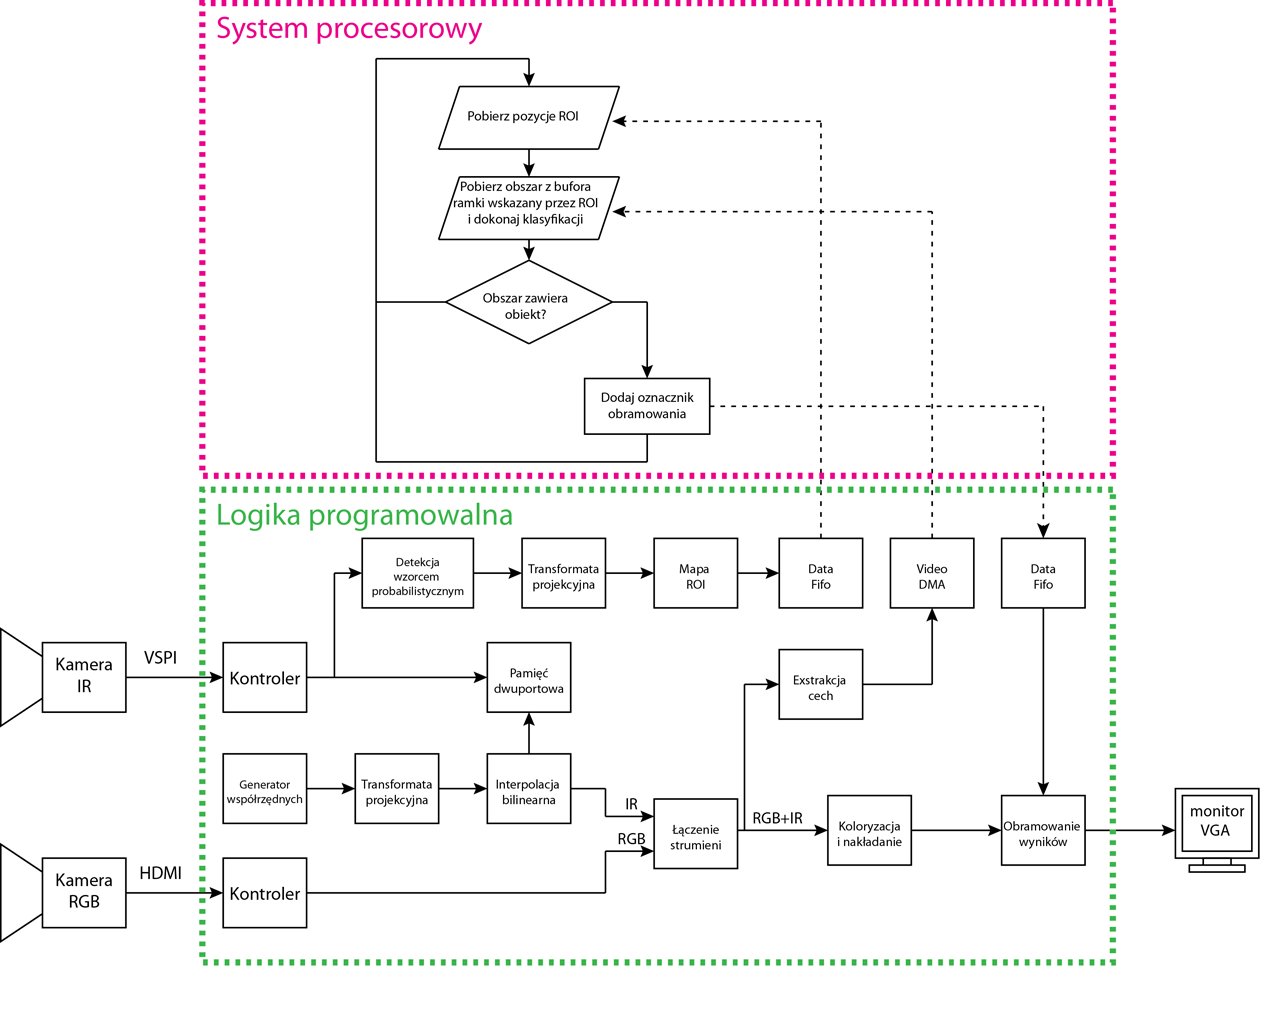
\includegraphics[width=1\textwidth]{images/system}
    \caption{Schemat blokowy systemu detekcji.}
    \label{fig:systemwizyjny}
\end{figure}

Programowalna logika:
\begin{itemize}
\item Akwizycja Obrazu poprzez HDMI (RGB) i VoSPI (IR),
\item Transformata projekcyjna i interpolacja obrazu IR,
\item Nałożenie i synchronizacja obrazu IR do obrazu RGB,
\item Prezentacja wyników,
\item Detekcja kandydatów za pomocą wzorca probabilistycznego.
\end{itemize}
System Procesorowy:
\begin{itemize}
\item konfiguracja parametrów systemu wizyjnego w logice programowalnej poprzez interfejs AXI-Lite,
\item Klasyfikacja obszarów wytypowanych przez wzorzec probabilistyczny,
\item Generowanie oznaczników.
\end{itemize}

\section{Opis modułów}
\subsection{Kontroler kamery IR}
Pobiera obraz z kamery poprzez interfejs VoSPI który następnie zostaje zapisany do dwuportowej pamięci BRAM. Kontroler na początku pracy wystawia pin CS (ang. Chip Select) w stan niski a po chwili rozpoczyna transmisję poprzez taktowanie zegarem SCK. Kamera na reaguje na opdające zbocze zegara i wystawia kolejny bit danych na swoim porcie MISO. Strumień VoSPI składa się z 63 pakietów na ramkę obrazu. Pakiet rozpoczyna identyfikator składający się z numeru linii oraz sumy CRC pakietu (2 bajty na numer linii i 2 na sumę). Dane pakietu stanowi 160 bajtów – po dwa bajty na piksel w linii. Dane są przesyłane w 14-bitową wartość piksela oraz 2 zera wypełnienia. W przypadku niepoprawnej ramki numer identyfikator przyjmuje wartość xFxx. Ostatnie trzy pakiety stanowią telemetrie i są ignorowane.

\subsection{Transformata projekcyjna}
Moduł zamienia współrzędne z układu odniesienia kamery RGB odpowiadającym im na obrazie IR. Na wejściu podawany jest strumień AXI4-Stream zawierający timingi oraz 12 bitowe współrzędne X i Y. Moduł realizuję operację: 

\begin{equation}
\begin{bmatrix}
u_n & v_n & n
\end{bmatrix} 
= 
\begin{bmatrix}
x & y & 1
\end{bmatrix}
T
\end{equation}

\begin{equation}
u = \frac{u_n}{n}
\end{equation}

\begin{equation}
v = \frac{v_n}{n}
\end{equation}

Moduł wystawia na wyjściu strumień timingów, 12 bitowe wartości U i V oraz ich części ułamkowe w U\_fraction i V\_fraction (14bitów). W module zostały wykorzystane 34 z 80 dostępnych w układzie Zynq procesorów DSP48 do wykonania operacji arytmetycznych. Najwięcej zasobów jest pochłonięte przez IP core dzielarki dostarczony od producenta układu. Do implementacji jednej dzielarki zostało wykorzystane14 modułów DSP. Dzielenie nie odbywa się w pełni potokowo. Użyty w dzielarce algorytm High\_Radix wymaga zatrzymanie strumienia na czas obliczeń. Jednak dzięki zastosowaniu wyższej częstotliwości niż zegar pikseli obrazu RGB oraz bufora (250 MHz) nie stanowi to wąskiego gardła systemu. Macierz T jest zapisana  w dziewięciu 32 bitowych rejestrach i konfigurowalna poprzez interfejs AXI4-Lite. Elementy macierzy są 25 liczbami w notacji stałoprzecinkowej: 1 bit znaku 10 – część całkowita, 14 – część ułamkowa.



\subsection{Interpolacja bilinearna}
Prosty moduł przeznaczony głównie do powiększania obrazów. PoModuł ma za zadanie pobrać z pamięci dwuportowej obrazu IR wartość piksela wskazaną na wejściu układu i wystawić na wyjście. Podobnie jak reszta systemu używa AXI4-Stream do przekazywania danych między poszczególnymi modułami. Dane na wejściu to współrzędne U i V oraz ich części ułamkowe U\_fraction i V\_fraction. Moduł został wyposażony w 4 rejestry w których przechowywane są współrzędne oraz wartości 4 ostatnio użytych pikseli. Zabieg ten znacznie redukuje ilość potrzebnych zapytań do pamięci. Podczas powiększania obrazów jest duża szansa że kolejne koordynaty na wejściu UV odwołują się do tych samych czterech otaczających ich pikseli. W module jest sprawdzane czy w pamięci już są wartości z koordynatów [U,V], [U+1,V] [U,V+1], [U+1,V+1]. Jeżeli któregoś piksela brakuje jest on pobierany z pamięci i zapisywany w rejestrze przechowującym niepotrzebny piksel. Jeżeli wszystkie koordynaty się zgadzają , obliczana jest wartość piksela wyjściowego z wzoru \ref{equ:bilinear}.  
\begin{equation}\label{equ:bilinear}
Ir = A(1-U_f)(1-V_f)+BU_f(1-V_f)+C(1-U_f)V_f+ D U_fV_f
\end{equation}
\noindent gdzie: $ A, B, C ,D $odpowiadają wartościom pikseli w [U,V], [U+1,V] [U,V+1], [U+1,V+1] a $ Ir $ to wartość wyjściowa piksela wyjściowego. $U_f$ i $V_f$ stanowią U\_fraction i V\_fraction.

Moduł działa strumieniowo. W przypadku gdy jest wymagana aktualizacja rejestrów strumień jest wstrzymywany.
biera wartość 4 otaczających, podanych na wejściu punktu, pikseli z BRAM i na ich bazie jest wykonywana interpolacja. Moduł zapamiętuje 4 ostatnio użyte piksele które są na bieżąco aktualizowane wraz z zmianą położenia punktu wejściowego na obrazie IR.
\subsection{Łączenie strumieni}
Moduł posiada dwa wejścia dla obrazu. Jeden strumień jest głównym i do niego jest dołączany drugi strumień. Do synchronizacja strumieni została wykorzystana możliwość AXI4-Strem do wstrzymania transmisji. Piksele z dołączanego strumienia są odrzucane do momentu pojawienia się sygnału SOF. W momencie pojawienia się sygnału SOF w strumieniu głównym transmisja zostaje wznowiona, pod kontrolą strumienia wyjściowego. Po przejciu całej ramki strumienie są ponownie synchronizowane.  
\subsection{Koloryzacja i nakładanie}
Strumień RGBIR zostaje połączone w jeden obraz. Obraz IR zostaje poddany koloryzacji na podstawie 12-bitowego LUT i nałożony w proporcjach 50 na 50 z obrazem RGB. Na wyjciu jest podany 24 bitowy strumień RGB.

\subsection{Obramowanie wyników}
Moduł dodaje do obrazu podanego na strumień wejściowy ramkę która następnie jest podawana dalej strumieniem wyjściowym. Parametry ramki są ustawiane przez dwa 32 bitowe rejestry. Pierwszy, -position\_reg-, zawiera pozycję gdzie ma się znajdować ramka na obrazie (lewy górny róg ramki), drugi -parameters\_reg- rejestr odpowiada za kolor i wielkość ramki. Rejestry są konfigurowane poprzez AXI4-Lite.

\section{System procesorowy}

System procesorowy spełnia dwa podstawowe zadania: konfiguracja modułów zawartych w logice programowalnej za pomocą interfejsu AXI4-Lite takich jak macierz projekcji, wartość progu binaryzacji i wartość progu mocy dopasowania dla modułu DPM, wzmocnienie oraz offset modułu normalizacji sygnału IR. Pozwala on również na zapisanie na karcie SD aktualną ramkę bądź pozytywnie sklasyfikowany obraz okna detekcyjnego, jak i obrazu do przeprowadzenia kalibracji.

Drugim podstawowym zadaniem jest przeszukanie listy kandydatów w celu znalezienia tego z największą mocą dopasowania, wyliczenie cech HOG i klasyfikacji SVM. Oryginalny rozmiar okna detekcji w układzie kamery IR wynosi 16x40 zaś na obrazie RGBIR analizowane jest okno 80x192 piksele. Okno jest podzielone na 60 komórek o wielkości 16x16 pikseli. Następnie są obliczane gradienty oraz histogram dla każdej komórki. Wykorzystany jest histogram ważony o 9 przedziałach. Do każdego histogramu jest przypisany dodatkowo suma kwadratów wszystkich wartości przedziałów. Następnie komórki są łączone w bloki 2 na 2 w obrębie którego dokonuje się normalizacji wykorzystując wcześniej obliczone sumy kwadratów. Bloki nakładają się na siebie dając w sumie 44 bloki. Suma histogramów z wszystkich bloków tworzy 1584 elementowy wektor cech. Wektor jest przemnożony przez wektor beta uzyskany w procesie nauczania SVM i dodany bias. Jeżeli uzyskany wynik jest większy od 0 badane okno zostaje sklasyfikowane z wynikiem pozytywnym.

